%%
% Template for Assignment Reports
% 
%

\documentclass{article}

\usepackage{fancyhdr} % Required for custom headers
\usepackage{lastpage} % Required to determine the last page for the footer
\usepackage{extramarks} % Required for headers and footers
\usepackage{graphicx,color}
\usepackage{anysize}
\usepackage{amsmath}
\usepackage{natbib}
\usepackage{caption}
\usepackage{hyperref}
\usepackage{listings}
\usepackage{float}
\usepackage{lipsum}  
\usepackage{xcolor}
\usepackage{subcaption}
\usepackage{listings}
\usepackage{color}

\definecolor{dkgreen}{rgb}{0,0.6,0}
\definecolor{gray}{rgb}{0.5,0.5,0.5}
\definecolor{mauve}{rgb}{0.58,0,0.82}

\lstset{frame=tb,
  language=Java,
  aboveskip=3mm,
  belowskip=3mm,
  showstringspaces=false,
  columns=flexible,
  basicstyle={\small\ttfamily},
  numbers=none,
  numberstyle=\tiny\color{gray},
  keywordstyle=\color{blue},
  commentstyle=\color{dkgreen},
  stringstyle=\color{mauve},
  breaklines=true,
  breakatwhitespace=true,
  tabsize=3
}

% Margins
%\topmargin=-0.45in
%\evensidemargin=0in
%\oddsidemargin=0in
\textwidth=6.5in
%\textheight=9.0in
%\headsep=0.25in 

\linespread{1.0} % Line spacing

\definecolor{codegreen}{rgb}{0,0.6,0}
\definecolor{codegray}{rgb}{0.5,0.5,0.5}
\definecolor{codepurple}{rgb}{0.58,0,0.82}
\definecolor{backcolour}{rgb}{0.95,0.95,0.92}

\lstdefinestyle{mystyle}{
    backgroundcolor=\color{backcolour},   
    commentstyle=\color{codegreen},
    keywordstyle=\color{magenta},
    numberstyle=\tiny\color{codegray},
    stringstyle=\color{codepurple},
    basicstyle=\ttfamily\footnotesize,
    breakatwhitespace=false,         
    breaklines=true,                 
    captionpos=b,                    
    keepspaces=true,                 
    numbers=left,                    
    numbersep=5pt,                  
    showspaces=false,                
    showstringspaces=false,
    showtabs=false,                  
    tabsize=2
}

\lstset{style=mystyle}

%%------------------------------------------------
%% Image and Listing code
%%------------------------------------------------
%%sw \includecode{caption for table of listings}{caption for reader}{filename}
\newcommand{\includecode}[3]{\lstinputlisting[float,floatplacement=H, caption={[#1]#2}, captionpos=b, frame=single]{#3}}


%%sw \includescalefigure{label}{short caption}{long caption}{scale}{filename}
\newcommand{\includescalefigure}[5]{
\begin{figure}[htb]
\centering
\includegraphics[width=#4\linewidth]{#5}
\captionsetup{width=.8\linewidth} 
\caption[#2]{#3}
\label{#1}
\end{figure}
}

%%sw \includefigure{label}{short caption}{long caption}{filename}
\newcommand{\includefigure}[4]{
\begin{figure}[htb]
\centering
\includegraphics{#4}
\captionsetup{width=.8\linewidth} 
\caption[#2]{#3}
\label{#1}
\end{figure}
}




%%------------------------------------------------
%% Parameters
%%------------------------------------------------
% Set up the header and footer
\pagestyle{fancy}
\lhead{\authorName} % Top left header
\chead{\moduleCode\ - \assignmentTitle} % Top center header
\rhead{\firstxmark} % Top right header
\lfoot{\lastxmark} % Bottom left footer
\cfoot{} % Bottom center footer
\rfoot{Page\ \thepage\ of\ \pageref{LastPage}} % Bottom right footer
\renewcommand\headrulewidth{0.4pt} % Size of the header rule
\renewcommand\footrulewidth{0.4pt} % Size of the footer rule
\setlength\parindent{0pt} % Removes all indentation from paragraphs

\newcommand{\assignmentTitle}{Final Project} % Assignment title
\newcommand{\moduleCode}{CSU44061} 
\newcommand{\moduleName}{Machine Learning} 
\newcommand{\authorName}{Adriana\ Hrabowych} % Your name
\newcommand{\authorID}{19304296} % Your student ID
\newcommand{\reportDate}{\printDate}

%%------------------------------------------------
%%	Title Page
%%------------------------------------------------
\title{
\vspace{-1in}
\begin{figure}[!ht]
\flushleft

\includegraphics[width=0.4\linewidth]{reduced-trinity.png}
\end{figure}
\vspace{-0.5cm}
\hrulefill \\
\vspace{0.5cm}
\textmd{\textbf{\moduleCode\ \moduleName}}\\
\textmd{\textbf{\assignmentTitle}}\\
\vspace{0.5cm}
\hrulefill \\
}

\author{\textbf{\authorName,\ \authorID}}

\date{\today}



%%------------------------------------------------
%% Document
%%------------------------------------------------
\begin{document}
\lstset{language=Java, captionpos=b, frame=single, keywordstyle=\color{black}\bfseries, stringstyle=\ttfamily}
\captionsetup{width=.8\linewidth} 

\maketitle


%%------------------------------------------------

\section{Part 1}

\subsection{(i) Data Preprocessing}

In total there are 38 csv files as part of the dublin bikes dataset, all over 100,000 lines and spanning from mid 2018 to the end of 2023. The files are gone through either chronologically by station or just chronologically. The header for each of these files is:
\begin{center}
STATION ID,TIME,LAST UPDATED,NAME,BIKE STANDS,AVAILABLE BIKE STANDS,AVAILABLE BIKES,STATUS,ADDRESS,LATITUDE,LONGITUDE
\end{center}

For these models, 'bike usage' is defined as the number of bikes taken from a station per day. Bikes being put back are ignored as its assumed that 'usage' has been logged previously when the bike was first taken.

Before starting any training, files are gone through one by one line by line in order to reduce and refine the data. First the data is separated into different dates, each day is represented by a class that contains its date, an array of stations, an array of station usages, and an array of \# of bikes at each station.

\begin{lstlisting}
class combinedStationTime:
  def __init__(self, date, station, bikes):
    self.date = date
    self.stations = [station]
    self.bikes = [bikes]
    self.usages = [0]
\end{lstlisting}
    
An array of these 'combinedStationTime's are maintained and each row of data either adds a new day or updates an existing one. If the current row's date already exists in the list, it will then check if that station is already in the list of station, if not it appends the station id, number of available bikes, and a usage of zero to each of the appropriate class lists. If that day already has that station within its list, it will then check if any bikes have been taken and increase the stations usage by 1 for each bike. Once all rows have been gone through, the average usage of all stations is calculated for each individual date.

The end result is a file called 'condenseddata.csv' which has a header of:
\begin{center}
DATE,AVG USAGE
\end{center}

When this data is read in and plotted in the main file the output is as shown in figure 1. There are a few gaps in the data, shown by horizontal connections over the gaps, as some dates weren't included in the files at all. There are also clear trends in the data, average usage drops significantly over holidays like new years and Christmas each year. It is obvious to see that usage fell drastically over the pandemic and has not recovered since.

\begin{center}
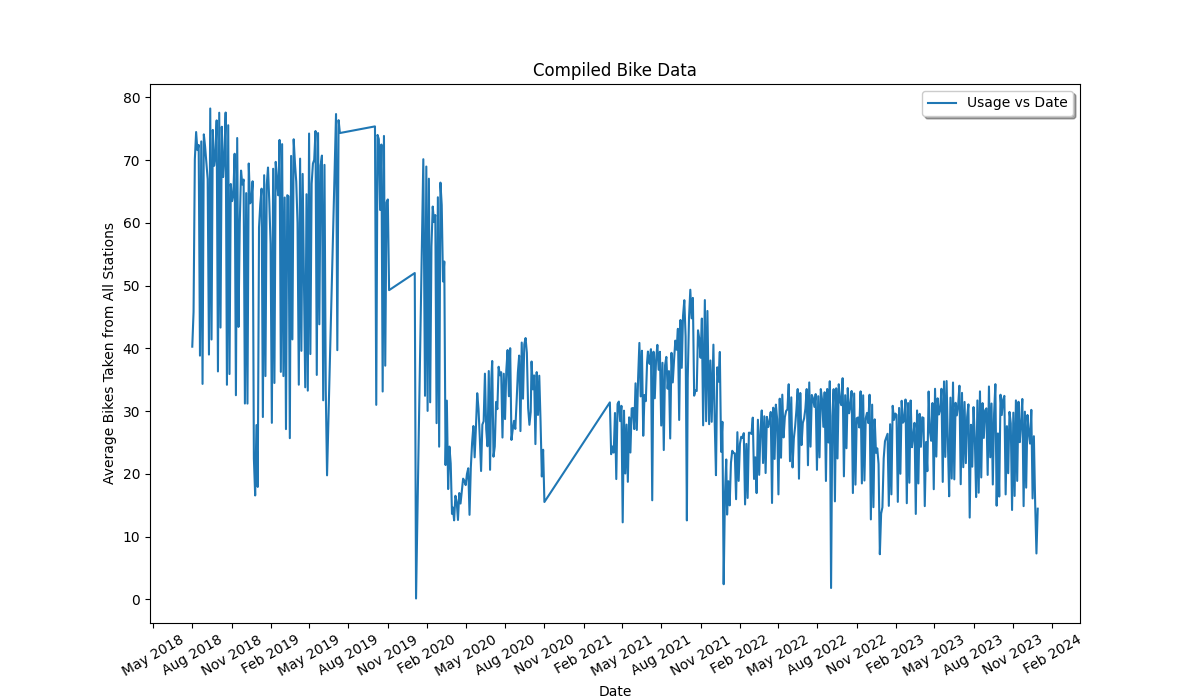
\includegraphics[width=1\linewidth]{CompiledData.png}
\end{center}
\captionof{figure}{A single line plot representing the average bike usage per day over the course of several years.}

\subsection{(ii) Machine Learning Methodology and Feature Engineering}

In order to see the impact of Covid on bike usage, a machine learning model will be trained only on pre-covid data and will then predict data over covid and postcovid periods. These predictions will be compared to the actual usage over those periods to see the full impact.

In this project a Linear Regression model is used. The first feature engineering that happened was to figure out the best date related variables to use. All of the date variables are in int format. The month and the type of weekday (Monday - Sunday) were the first variables considered as there are trends over months and weekdays with holidays and weekends. The year can be useful as there are trends as years go by, though with only 2 and a bit years of precovid data to train on the usefulness of this variable was unsure. Additionally the day was considered to potentially not be too useful as there are holidays on different days in every month so getting useful information by what day of the month it is would be hard. Four different Linear Regression models were trained and tested: One using weekdays and months (w+m), one with w+m+years, one with w+m+days, and one with w+m+years+days. A dummy model with each set of variables was also trained and tested.

The results were that the r2 scores of the dummy models were all zero as it would just predict the mean value for each input. The r2 scores of the models pre-covid period predictions vs actual pre-covid period predictions were all similar, between 0.32 and 0.34. Although in both the models that used the day variable its coefficient was below 0.06 and so its influence is negligable. Though the inclusion of the year variable did raise the r2 score by 0.02, its inclusion when predicting over a larger course of time causes the model to overly rely on it with a large coefficient. This can be seen in figure two. So from this the only variables we will use for our final model is the month and weekday.

The next bit of feature engineering was to decide on the degree of the polynomial the model should have. This might seem strange as the features are categorical and not continuous but as they are represented by ints they can still be transformed. Additionally as the data is not linear, increasing the degree will help the model predict more accurately. The degrees chosen to test were 1, 2, 5, 7,  these were chosen as they represent a good spread and represent the typical range of degrees used in linear regression models.

\begin{center}
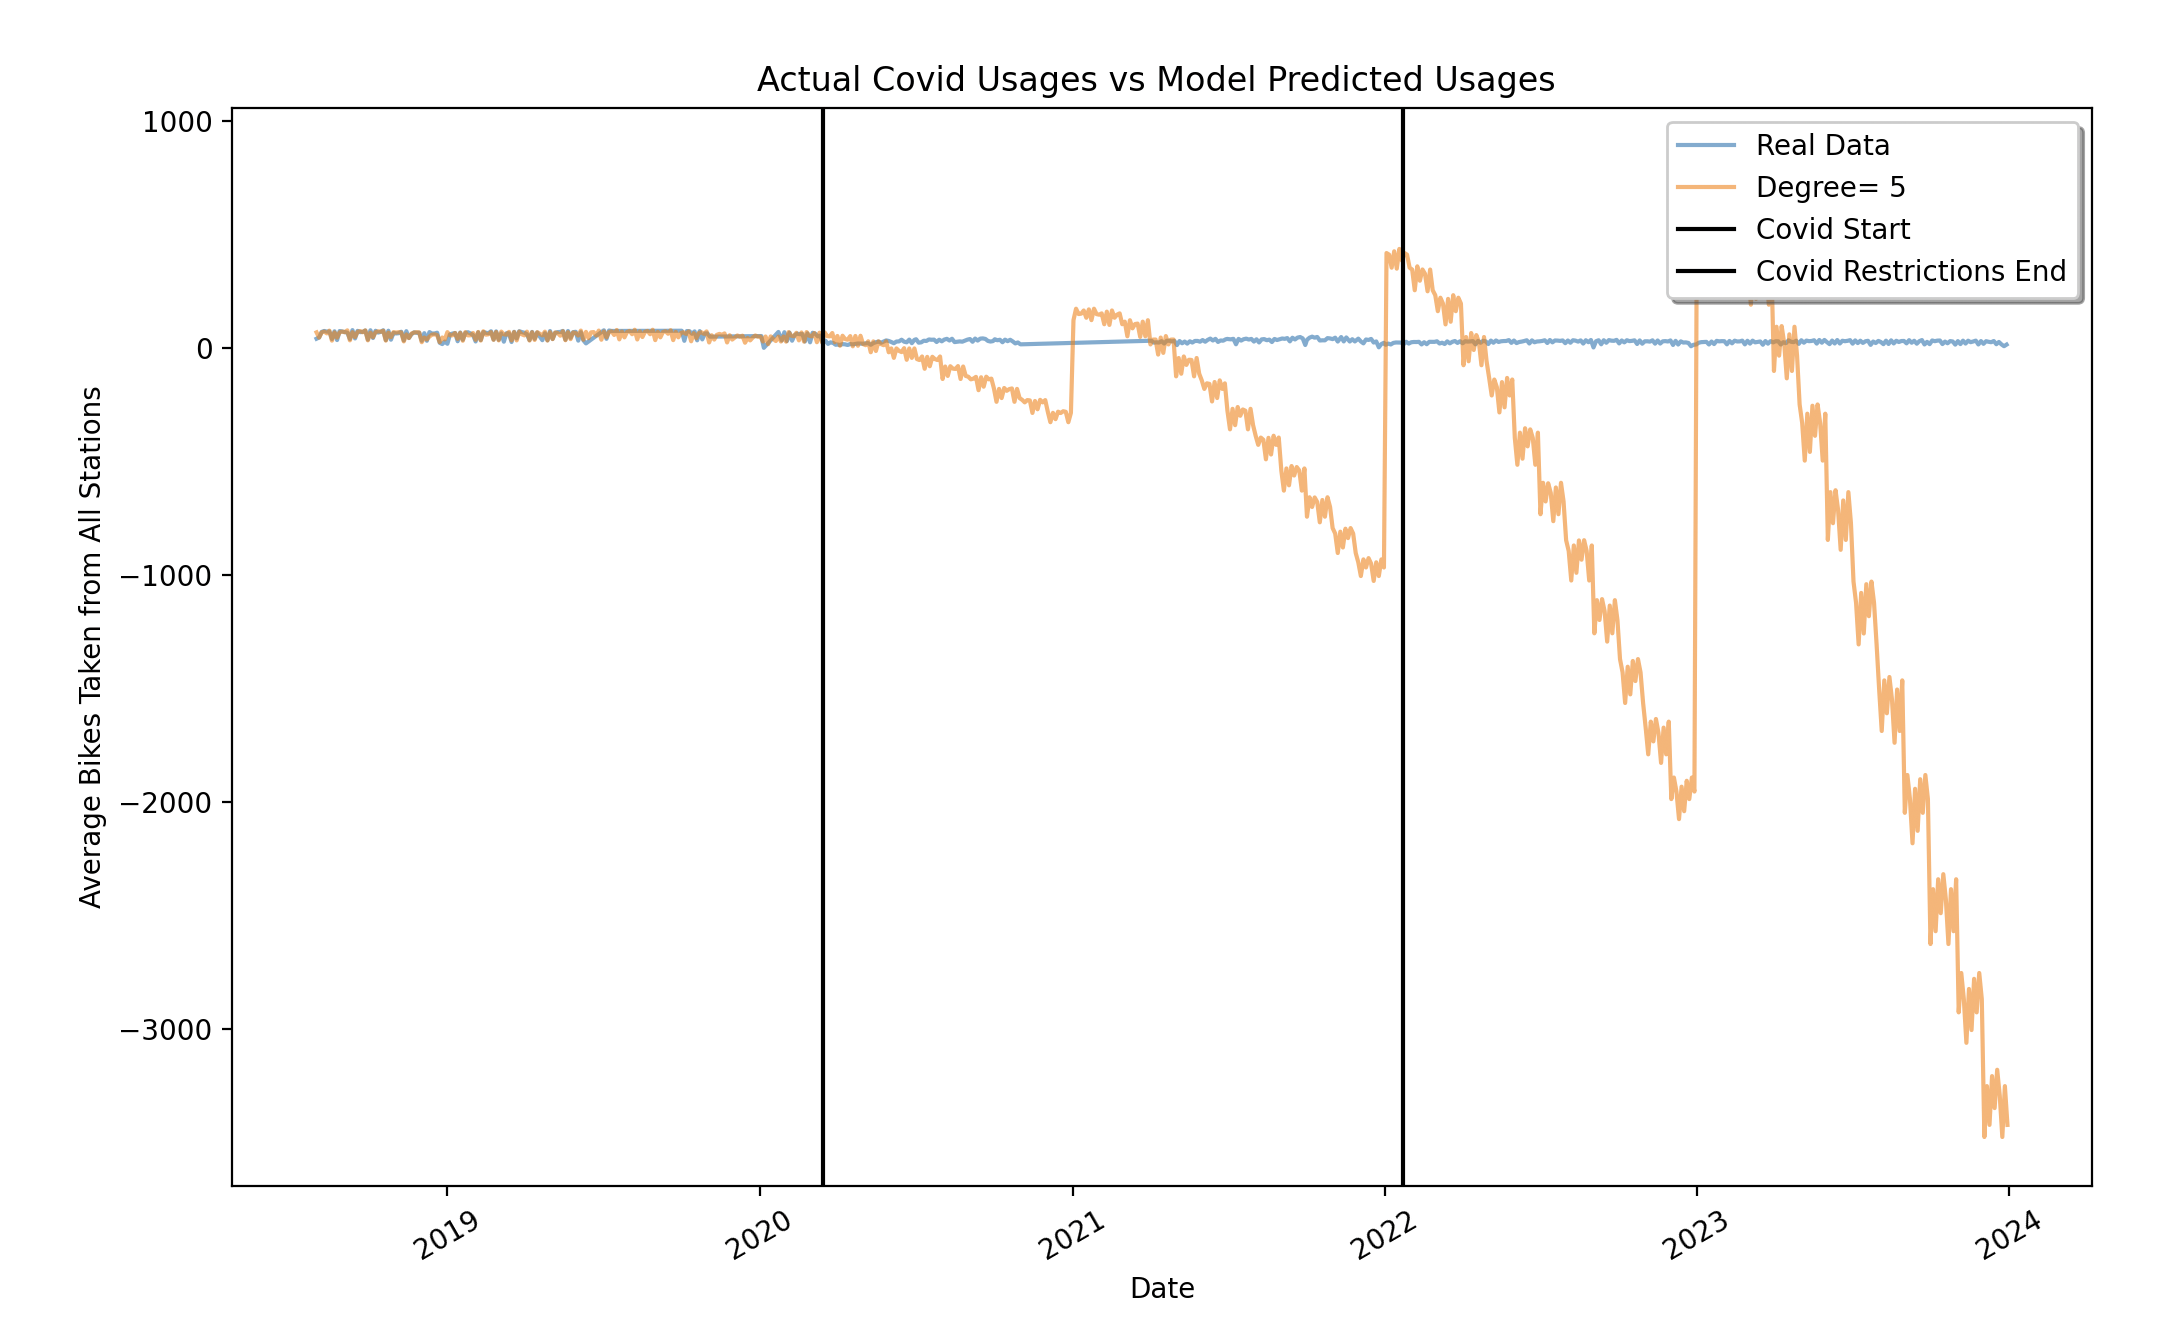
\includegraphics[width=1\linewidth]{failure.png}
\end{center}
\captionof{figure}{A graph of actual data vs predicted data over the entire time period. The predicted data is very inaccurate.}

The process of testing the different polynomial degrees was the same as feature engineering for the different variables, the graphs can be seen in figure 3. The r2 scores of each model were as follows:
\begin{center}
Degree 1	-	0.345 \newline
Degree 2	-	0.635\newline
Degree 5	-	0.683\newline
Degree 7	-	0.706\newline
\end{center}
Though the model with a degree of 7 performed the best, a model with that many parameters can be easily overfit, so instead for the final model a degree of five will be used.

\subsection{(iii) Evaluation}

The final model was a linear regression model that took in two variables (months and weekdays) to a polynomial degree of 5. This model was trained on pre-covid data and then was told to predict the entire timerange (including covid and post-covid time), this was plotted against the real values. This graph can be seen in figure 4. The model predicts the same values for each year, causing a repeating pattern. It can be seen from the graph that the actual pandemic usages and post pandemic usages were much lower than the predicted values. This shows that the pandemic clearly had a noticeable and still present impact on Dublin Bike usage.

There were many problems with the methodologies used this project. A Linear Regression model was not the best model to choose for this scenario, as it isn't complex enough and the variables are categorial which does not engage well with linear regression. An ARIMA model or any model that can work well with time series data would have been more effective at accurately predicting the usage. Originally, an ARIMA model was going to be used but unfortunately the writer could not get the packages to work on their Mac. Additionally, the models may have been more accurate if more variables were introduced other than time. This was not done due to time constraints.

\begin{figure} [H]
\centering
\begin{subfigure}{.49\linewidth}
  \centering
  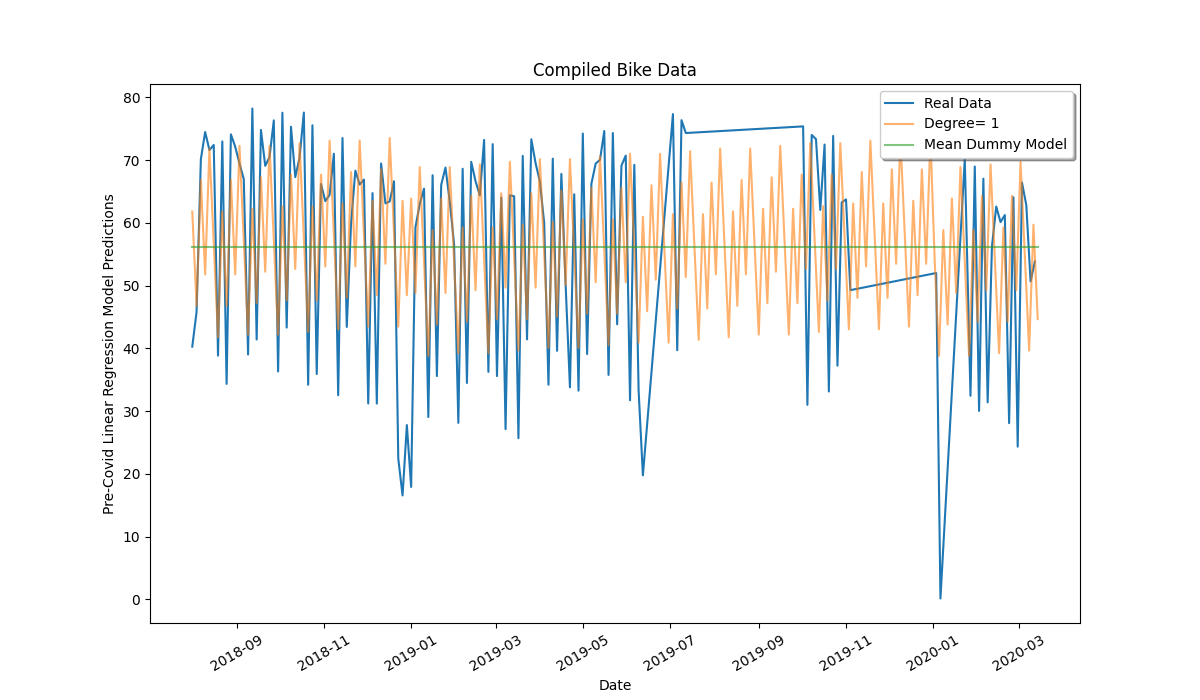
\includegraphics[width=\linewidth, height=6cm]{featuremodel1.png}
  \caption{Model with polynomial degree = 1 vs actual.}
  \label{fig:sub1}
\end{subfigure}%
\begin{subfigure}{.49\textwidth}
  \centering
  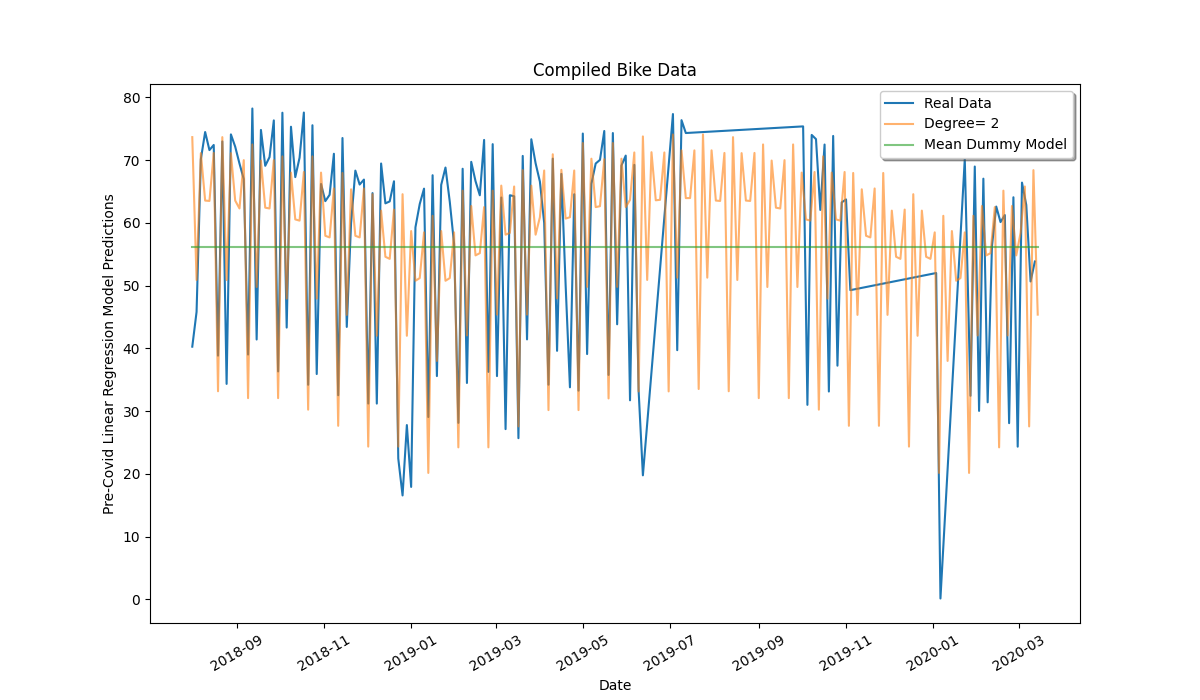
\includegraphics[width=\linewidth, height=6cm]{featuremodel2.png}
  \caption{Model with polynomial degree = 2 vs actual.}
  \label{fig:sub2}
\end{subfigure}
\label{fig:test}
\begin{subfigure}{.49\linewidth}
  \centering
  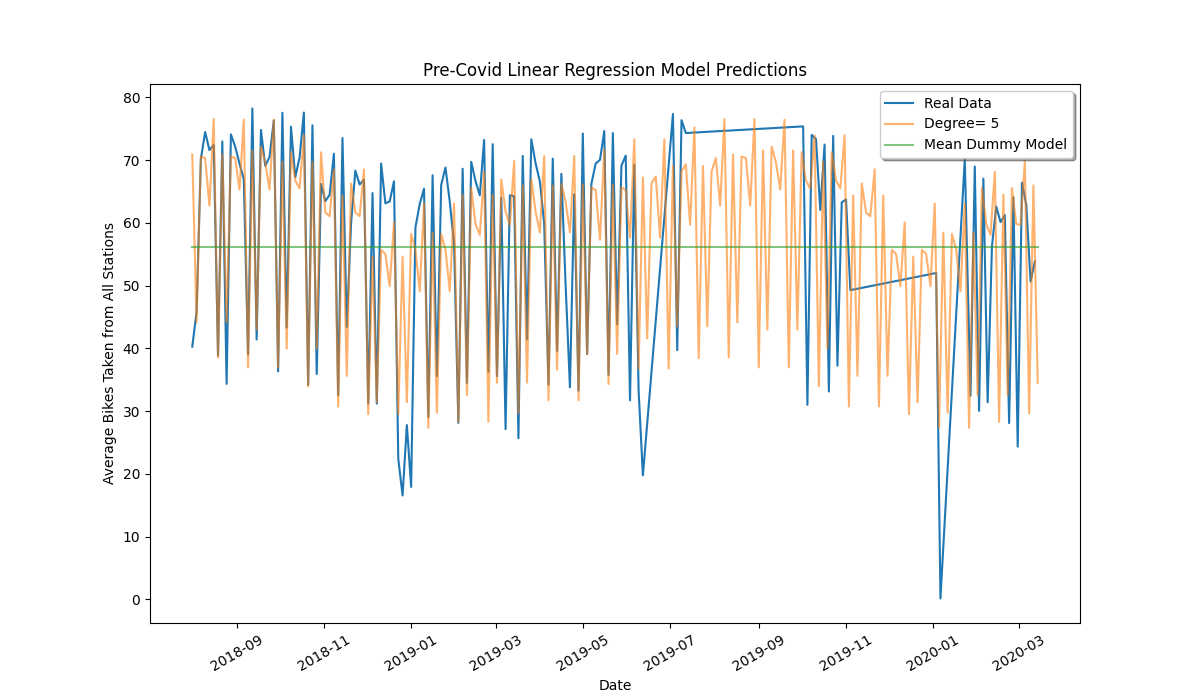
\includegraphics[width=\linewidth, height=6cm]{featuremodel5.png}
  \caption{Model with polynomial degree = 5 vs actual.}
  \label{fig:sub3}
\end{subfigure}%
\begin{subfigure}{.49\linewidth}
  \centering
  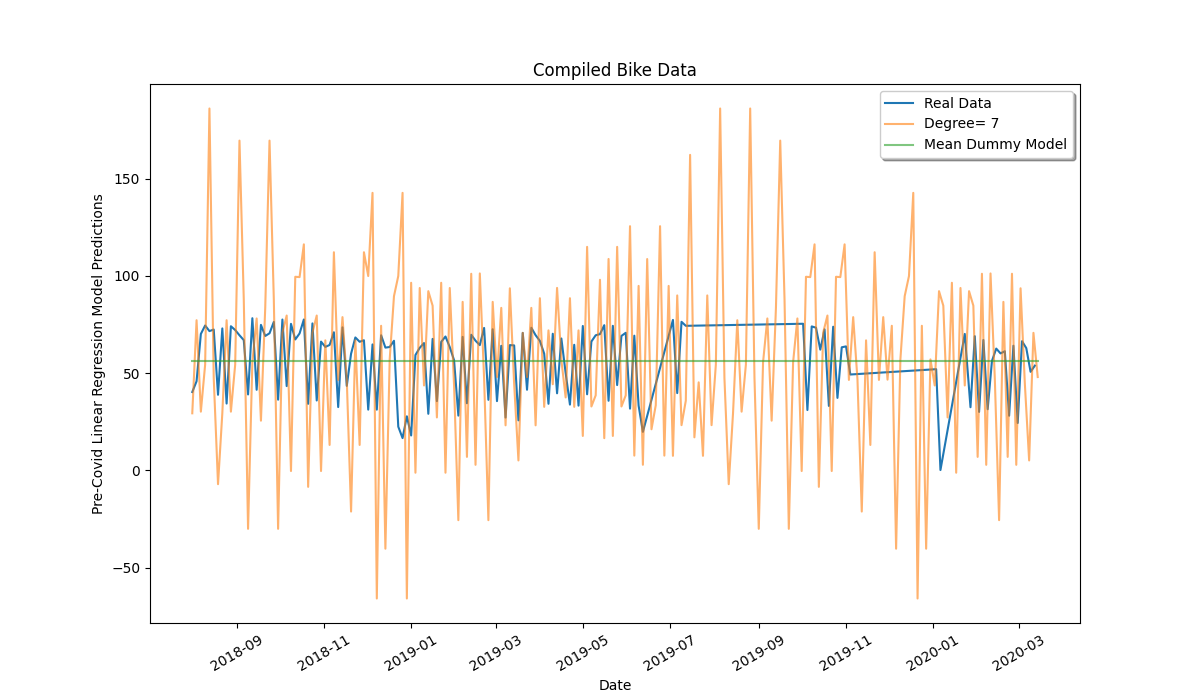
\includegraphics[width=\linewidth, height=6cm]{featuremodel7.png}
  \caption{Model with polynomial degree = 7 vs actual.}
  \label{fig:sub3}
\end{subfigure}%
\caption{A figure with four subfigures, each containing two plots. One is the plot of the actual average bike usage over pre covid dates and the other is a model prediction the average bike usage over pre covid dates. Each subfigure differs in the polynomial degree the variables in the models use. }
\label{fig:test}
\end{figure}

\section{Part 2}
\subsection{(i)}
An ROC curve is line that plots the true positive rate of a model against the false positive rate of a model at different classification thresholds. A classification threshold is the threshold that must be reached for a model to classify a point as positive. The formula for each rate are as follows:
\begin{center}
TPR = TP / (TP + FN)

FPR = FP / (FP + TN)
\end{center}
An ROC curve is considered better the closer the line is to an upside down L as it would mean that when the classification threshold is 1 the false positive rate is 0. A perfect model would have this L shape. The ROC curve for a baseline model is usually close to a perfectly diagonal line as the TPR usually equals the FPR. You would want to use an ROC curve over a classification accuracy metric to evaluate your models when its known that the data classifications are unequal in size. If the data is 99 percent class 1, then a baseline model that always predicts class 1 will have a very high accuracy, potentially better than a well fit model. Obviously, using this baseline model isn't good as it will have a lot of false class 1s. Using an ROC curve to analyze models can make it easier to see which models have the lowest number of false positives and highest true positives.

\begin{center}
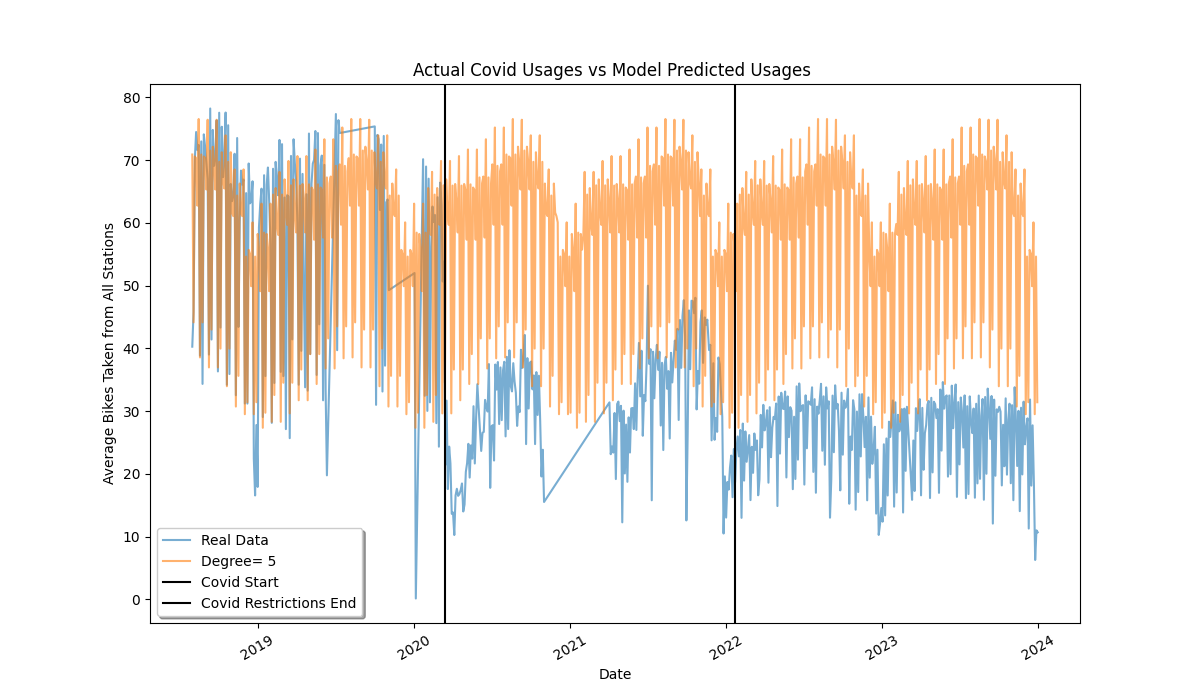
\includegraphics[width=1\linewidth]{covidDif5}
\end{center}
\captionof{figure}{A graph of actual data vs predicted data over the entire time period. The mode used was a linear regression model with a polynomial degree of five}

\subsection{(ii)}
Linear Regression models, as the name suggests, are meant to model linear relationships. If the data has a non-linear relationship (ex. a parabola shape) then a LR model will not be able to capture it accurately and would not give the most accurate predictions. This can be mitigated by increasing the number of features through polynomial transformations of existing features. With a polynomial degree of 2 for the features, the equation changes from a linear to a quadratic equation and can be used in a non-linear dataset.

This solution however can lead to a different problem, where too little data and too many parameters used in a LR model can cause the model to overfit the data and the outliers of the data become exaggerated in predictions. This can be solved in two ways, firstly by carefully selecting the number of parameters so that the model doesn't under or over fit. Secondly, before training normalize the data and potentially remove outliers so that theres less noise the begin with.

\subsection{(iii)}
Both types of kernels transform the data in some way. The kernel in a kernelized SVM is a function that transforms the training data into different forms depending on whats needed. There are several different types of kernels, the 'kernel trick' kernel for example will transform the data to a higher plane so that non-linear relationships can be represented linearly. In Convolutional Neural Networks a kernel is a filter that is applied to an input matrix to produce an output matrix, a typical CNN will use many different kernels to transform the data over many layers. A kernel can be any size smaller than the input matrix, and different kernel sizes can lead to the size of the input changing in the output. In image processing, kernels can be used to detect edges in an image. 

\subsection{(iv)}
In K-Fold Cross Validation the data is sampled over multiple times, this resampling is done to allow us to evaluate how the model performs generally. This is because if we were to only split and train and test once we'd only get one score, this score might be affected by an odd splitting of training/testing or some other bias. But, in K-fold our final score is the K\# of score's from each fold / K, aka the average scores over K folds. As this is an average its easier to trust, even if one those folds got a really good or bad score by chance its evened out by the other scores and so therefore the end score is more representative of the model. For example, if you trained and tested you model and got a score of 0.80 accuracy you would assume the model is good and would use it over other models/hyper parameter combinations. But that score was an outlier, now every time you use the model the score is around 0.40. If you had used K-fold cross validation to begin with, with a K of five in this example, the score for that model would have been (0.4 * 4 + 0.8 / 5 = 0.48) which is quite low and would have given you the chance to explore different models.

It is not appropriate to use K-fold to cross validate when the datasets are very large as K-fold increases the computational time and power to train/test by K. Another scenario where K-fold isn't appropriate is in time-series data (like this project) as the order of the data is important and so the arbitrary K-splits and potentially predicting past dates than what was trained on would cause the scores to be inaccurate. 

\section{Appendix}
\lstinputlisting[language=Python]{../main.py}
\lstinputlisting[language=Python]{../readfiles.py}

\end{document}



